\subsection{Distribution of the attributes}
We generate the histogram for 9 attributes to find whether the attributes is normal distributed. We did not analysis the attributes X, Y, month and day since it is meaningless draw the histogram for them. From the histogram we can find that the FFMC, ISI and temp attributes seems to be like normal distributed. But others are not. 

\begin{figure}[!ht]
\centering
\begin{subfigure}[b]{.45\linewidth}
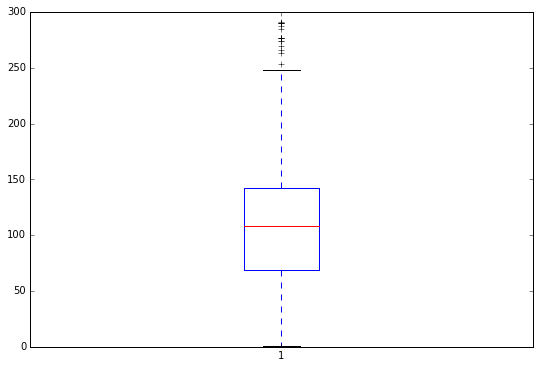
\includegraphics[width=\linewidth]{fig/hist/DMC.png}
\caption{DMC}\label{fig:mouse}
\end{subfigure}

\begin{subfigure}[b]{.45\linewidth}
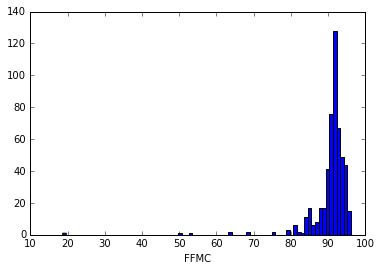
\includegraphics[width=\linewidth]{fig/hist/FFMC.png}
\caption{FFMC}\label{fig:gull}
\end{subfigure}
\begin{subfigure}[b]{.45\linewidth}
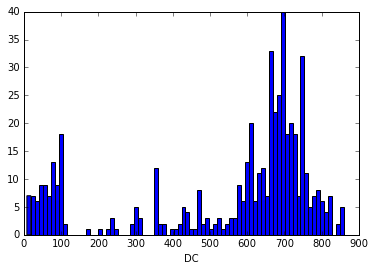
\includegraphics[width=\linewidth]{fig/hist/DC.png}
\caption{DC}\label{fig:tiger}
\end{subfigure}
\begin{subfigure}[b]{.45\linewidth}
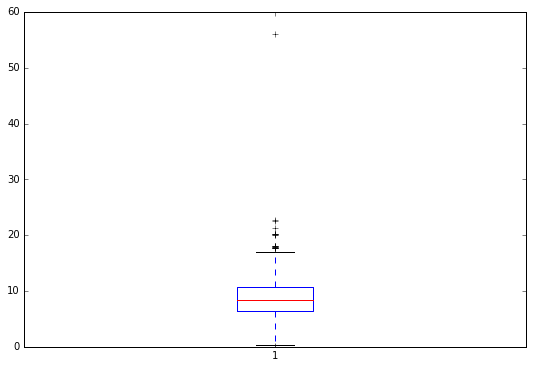
\includegraphics[width=\linewidth]{fig/hist/ISI.png}
\caption{ISI}\label{fig:tiger}
\end{subfigure}
\begin{subfigure}[b]{.45\linewidth}
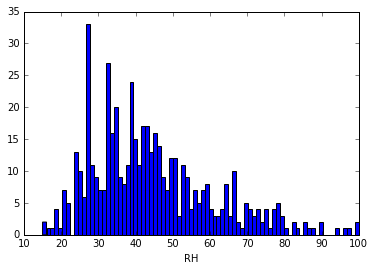
\includegraphics[width=\linewidth]{fig/hist/RH.png}
\caption{RH}\label{fig:tiger}
\end{subfigure}
\caption{Histogram 1}
\end{figure}

\begin{figure}[!ht]
\begin{subfigure}[b]{.45\linewidth}
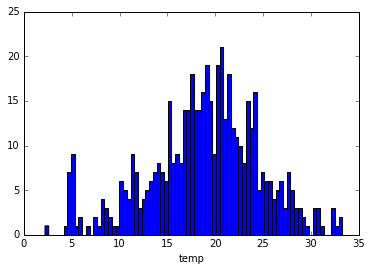
\includegraphics[width=\linewidth]{fig/hist/temp.png}
\caption{Temp}\label{fig:gull}
\end{subfigure}
\begin{subfigure}[b]{.45\linewidth}
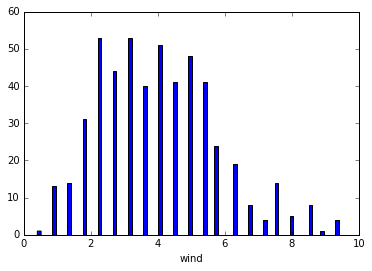
\includegraphics[width=\linewidth]{fig/hist/wind.png}
\caption{Wind}\label{fig:tiger}
\end{subfigure}
\begin{subfigure}[b]{.45\linewidth}
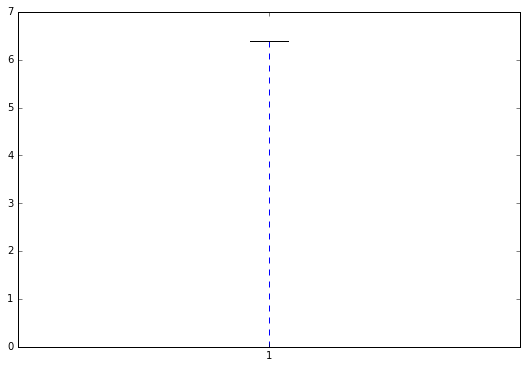
\includegraphics[width=\linewidth]{fig/hist/rain.png}
\caption{Rain}\label{fig:tiger}
\end{subfigure}
\begin{subfigure}[b]{.45\linewidth}
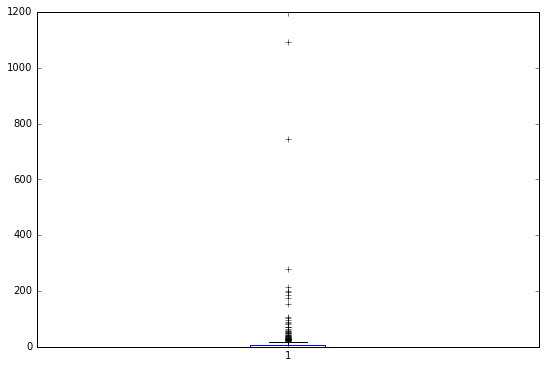
\includegraphics[width=\linewidth]{fig/hist/area.png}
\caption{Area}\label{fig:tiger}
\end{subfigure}
\caption{Histogram 2}
\end{figure}
